\chapter{Agile Software Development}\label{chapter3}
Agile methodologies are used by most of the software engineers today. These methodologies have been adapted into different agile frameworks providing clearer guidelines for the development process. This chapter explores if and how current agile frameworks take the sustainability impact of software into account and what agile frameworks already exist for creating more sustainable software. The frameworks inspected here are limited to team-level agile frameworks and as such will not take into account models such as Scrum at Scale, SAFe, and LeSS.

\section{Existing Agile Frameworks}
The most used agile frameworks are Scrum, Extreme programming, and Kanban with Scrum being the most utilized~\cite{empiricalstudyofagile}\cite{usageandperceptions}. This section explains these agile frameworks briefly. These frameworks are mostly focused on \gls{technicalsustainability} and as such were used to find ways to improve that sustainability aspect in the model proposed in this thesis.

\subsection{Scrum}\label{scrum}
Scrum has three roles: Scrum master, Product owner, and developer. The Scrum master makes sure that the scrum is followed correctly and helps the team be as effective as possible by helping other roles in scrum events. The product owner is responsible for maximizing the value of the product. The product owner has the vision for the product and communicates it to other members as well as the stakeholders. They also facilitate communication between stakeholders and the development team. Developers create the backlog for each sprint and do the actual development work.~\cite{scrumguide}

Scrum has events that should happen in every sprint. These events are Sprint planning, daily scrum, sprint review, and sprint retrospective. Planning is used to see what work is going to be done during the sprint. The daily scrum is a catch-up event each day for communicating what every member of the development team will be doing. Review is used to discuss what was accomplished during the sprint with the key stakeholders. Finally retrospective is used to discuss how the sprint went and what can be learned and implemented for the next sprint.~\cite{scrumguide}

Scrum also has artifacts which are the product backlog, sprint backlog, and an increment. The product backlog contains all the planned work for the product. Sprint backlog contains planned work for that sprint and an increment which is the version of the product being built after the sprint. The Scrum process is illustrated in Figure~\ref{scrumprocess}.~\cite{scrumguide}

Scrum does not take qualitative aspects of software such as stability or performance into account unless they are part of the requirements for some feature or the overall system~\cite{scrumguide}. Some requirements for these aspects could appear in the definition of done for some user stories if so defined by the product owner or if there is a requirement from the client for some functionality to be performed within certain time limit. Without external requirements, sustainability aspects are unlikely to be part of the definition of done for any user story.

\begin{figure}[H]
\caption{Scrum process~\cite{scrumWhatScrum}}
\label{scrumprocess}
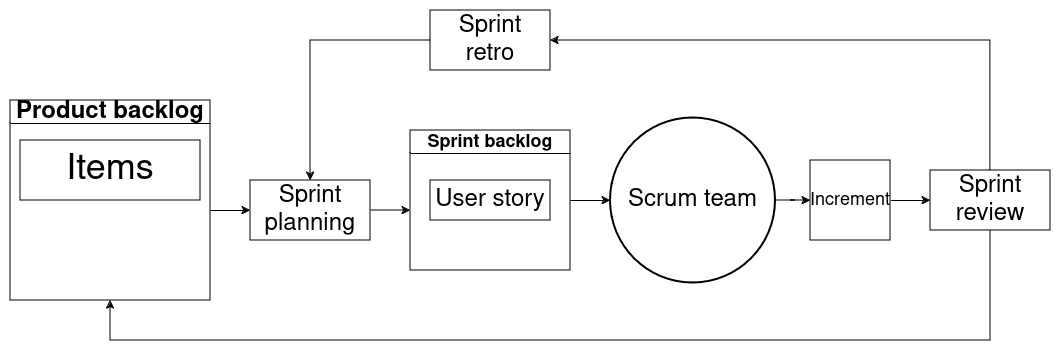
\includegraphics[width=\textwidth]{scrum.png}
\centering
\end{figure}

\subsection{Extreme programming}\label{xp}
Extreme programming is often more used in embedded domains where energy efficiency and performance have already been a concern for years due to hardware limitations~\cite{agilemethodsinembedded}. Extreme programming uses user stories to create a backlog like Scrum. Unlike Scrum, Extreme programming is more opinionated in how the actual development process is conducted. It enforces measures such as test-driven development, pair programming, enforced standards, and refactoring to ensure the quality of the software being produced. Extreme programming also imposes a 10-minute limit on build times for the software. In addition, extreme programming uses spikes which are simple throwaway programs to explore potential solutions to a complex or uncertain problem. The extreme programming process is illustrated in Figure~\ref{xpprocess}.~\cite{extremeprogrammingExtremeProgramming}

\begin{figure}[H]
\caption{Extreme programming project steps~\cite{extremeprogrammingFlowChart}}
\label{xpprocess}
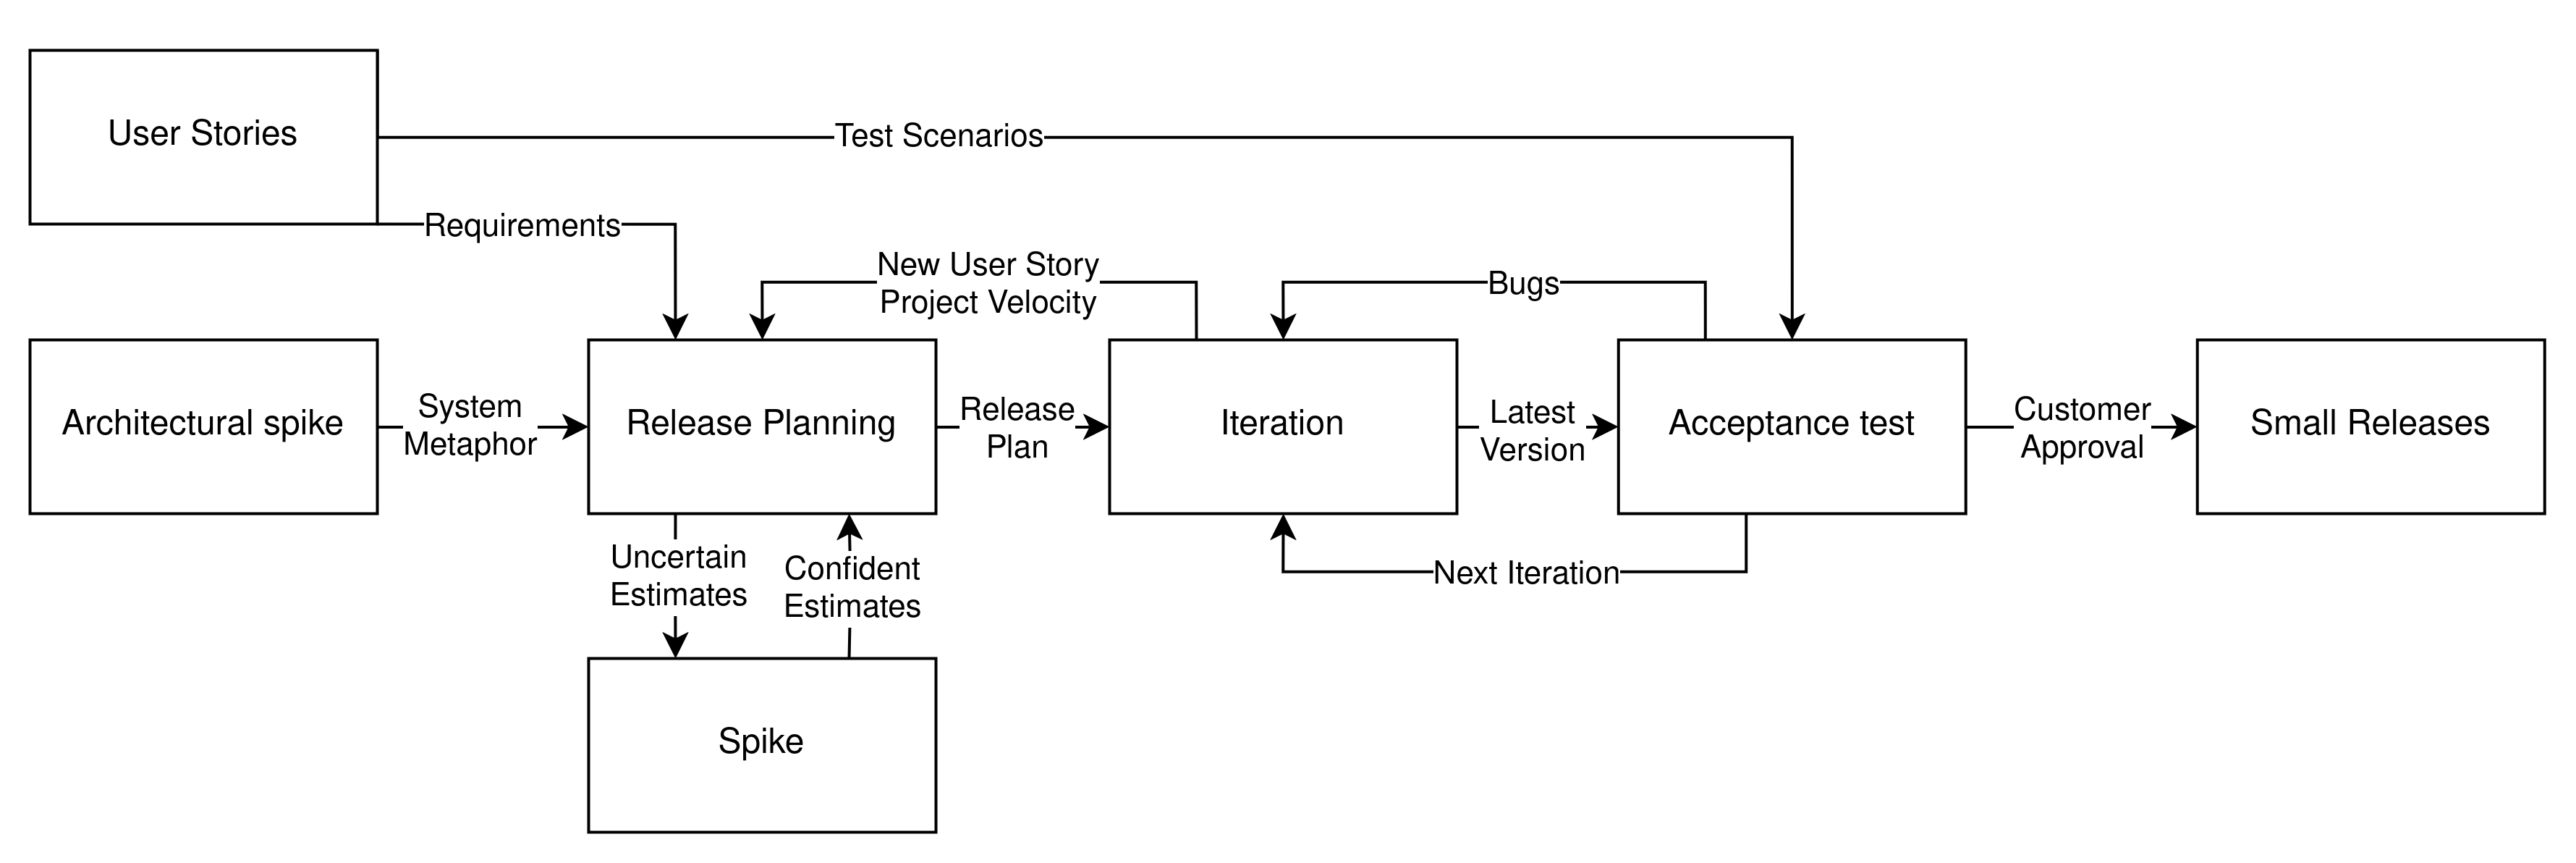
\includegraphics[width=\textwidth]{images/xp.png}
\centering
\end{figure}

\subsection{Kanban}\label{kanbanmethod}
Kanban is the simplest of the three most used Agile methodologies. Kanban can also refer to the Kanban board as a tool that is often used in other agile processes such as Scrum or Extreme programming. Kanban uses the Kanban board to keep track of the work. The Board is separated into different statuses of the tasks or user stories that are currently being done. Unlike Scrum, Kanban does not have specific roles for different members of the team. The Kanban board is shown in Figure \ref{kanban}.

\begin{figure}[H]
\caption{Kanban board}
\label{kanban}
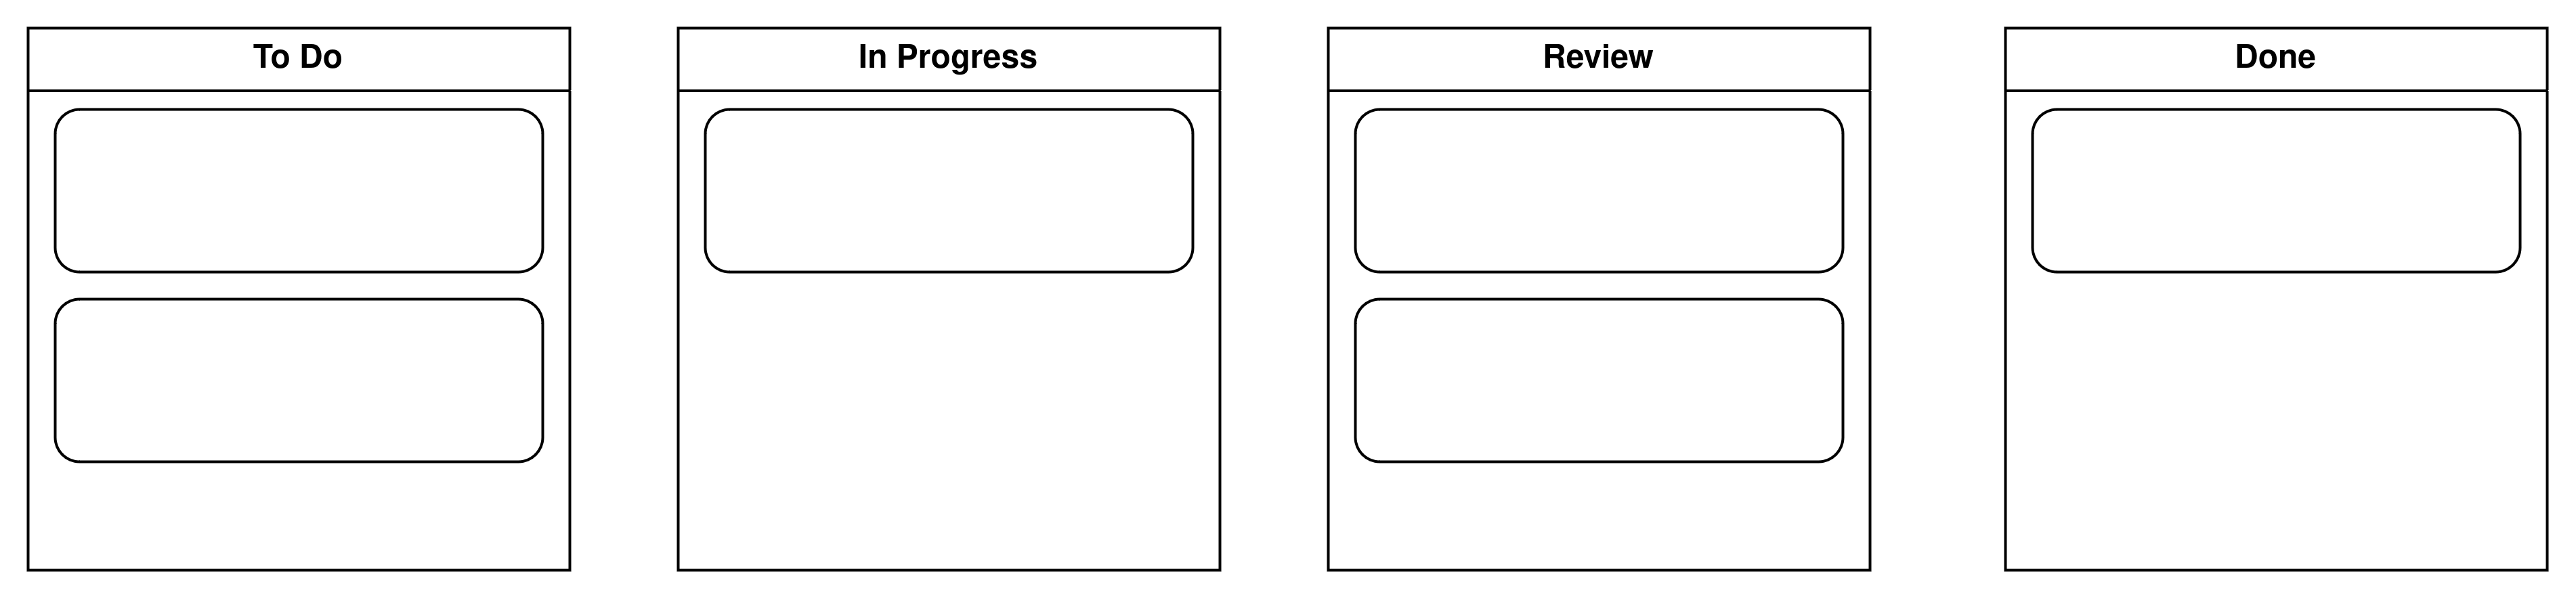
\includegraphics[width=\textwidth]{kanban}
\centering
\end{figure}

\section{Existing research for developing green software}
There is some existing research on developing software while taking into account its impact. This section explores three such development models.

\subsection{The Greensoft model}\label{greensoft}
The Greensoft model is a reference model for software engineering that takes into account the entire life cycle of a software product from development to end of life. It also presents metrics for measuring sustainability, procedures for different parties involved in the use of software, and tool recommendations for these parties. The overview of the Greensoft model is shown in Figure~\ref{greensoftoverview}.

\begin{figure}[H]
\caption{Overview of the Greensoft model~\cite{greensoft}}
\label{greensoftoverview}
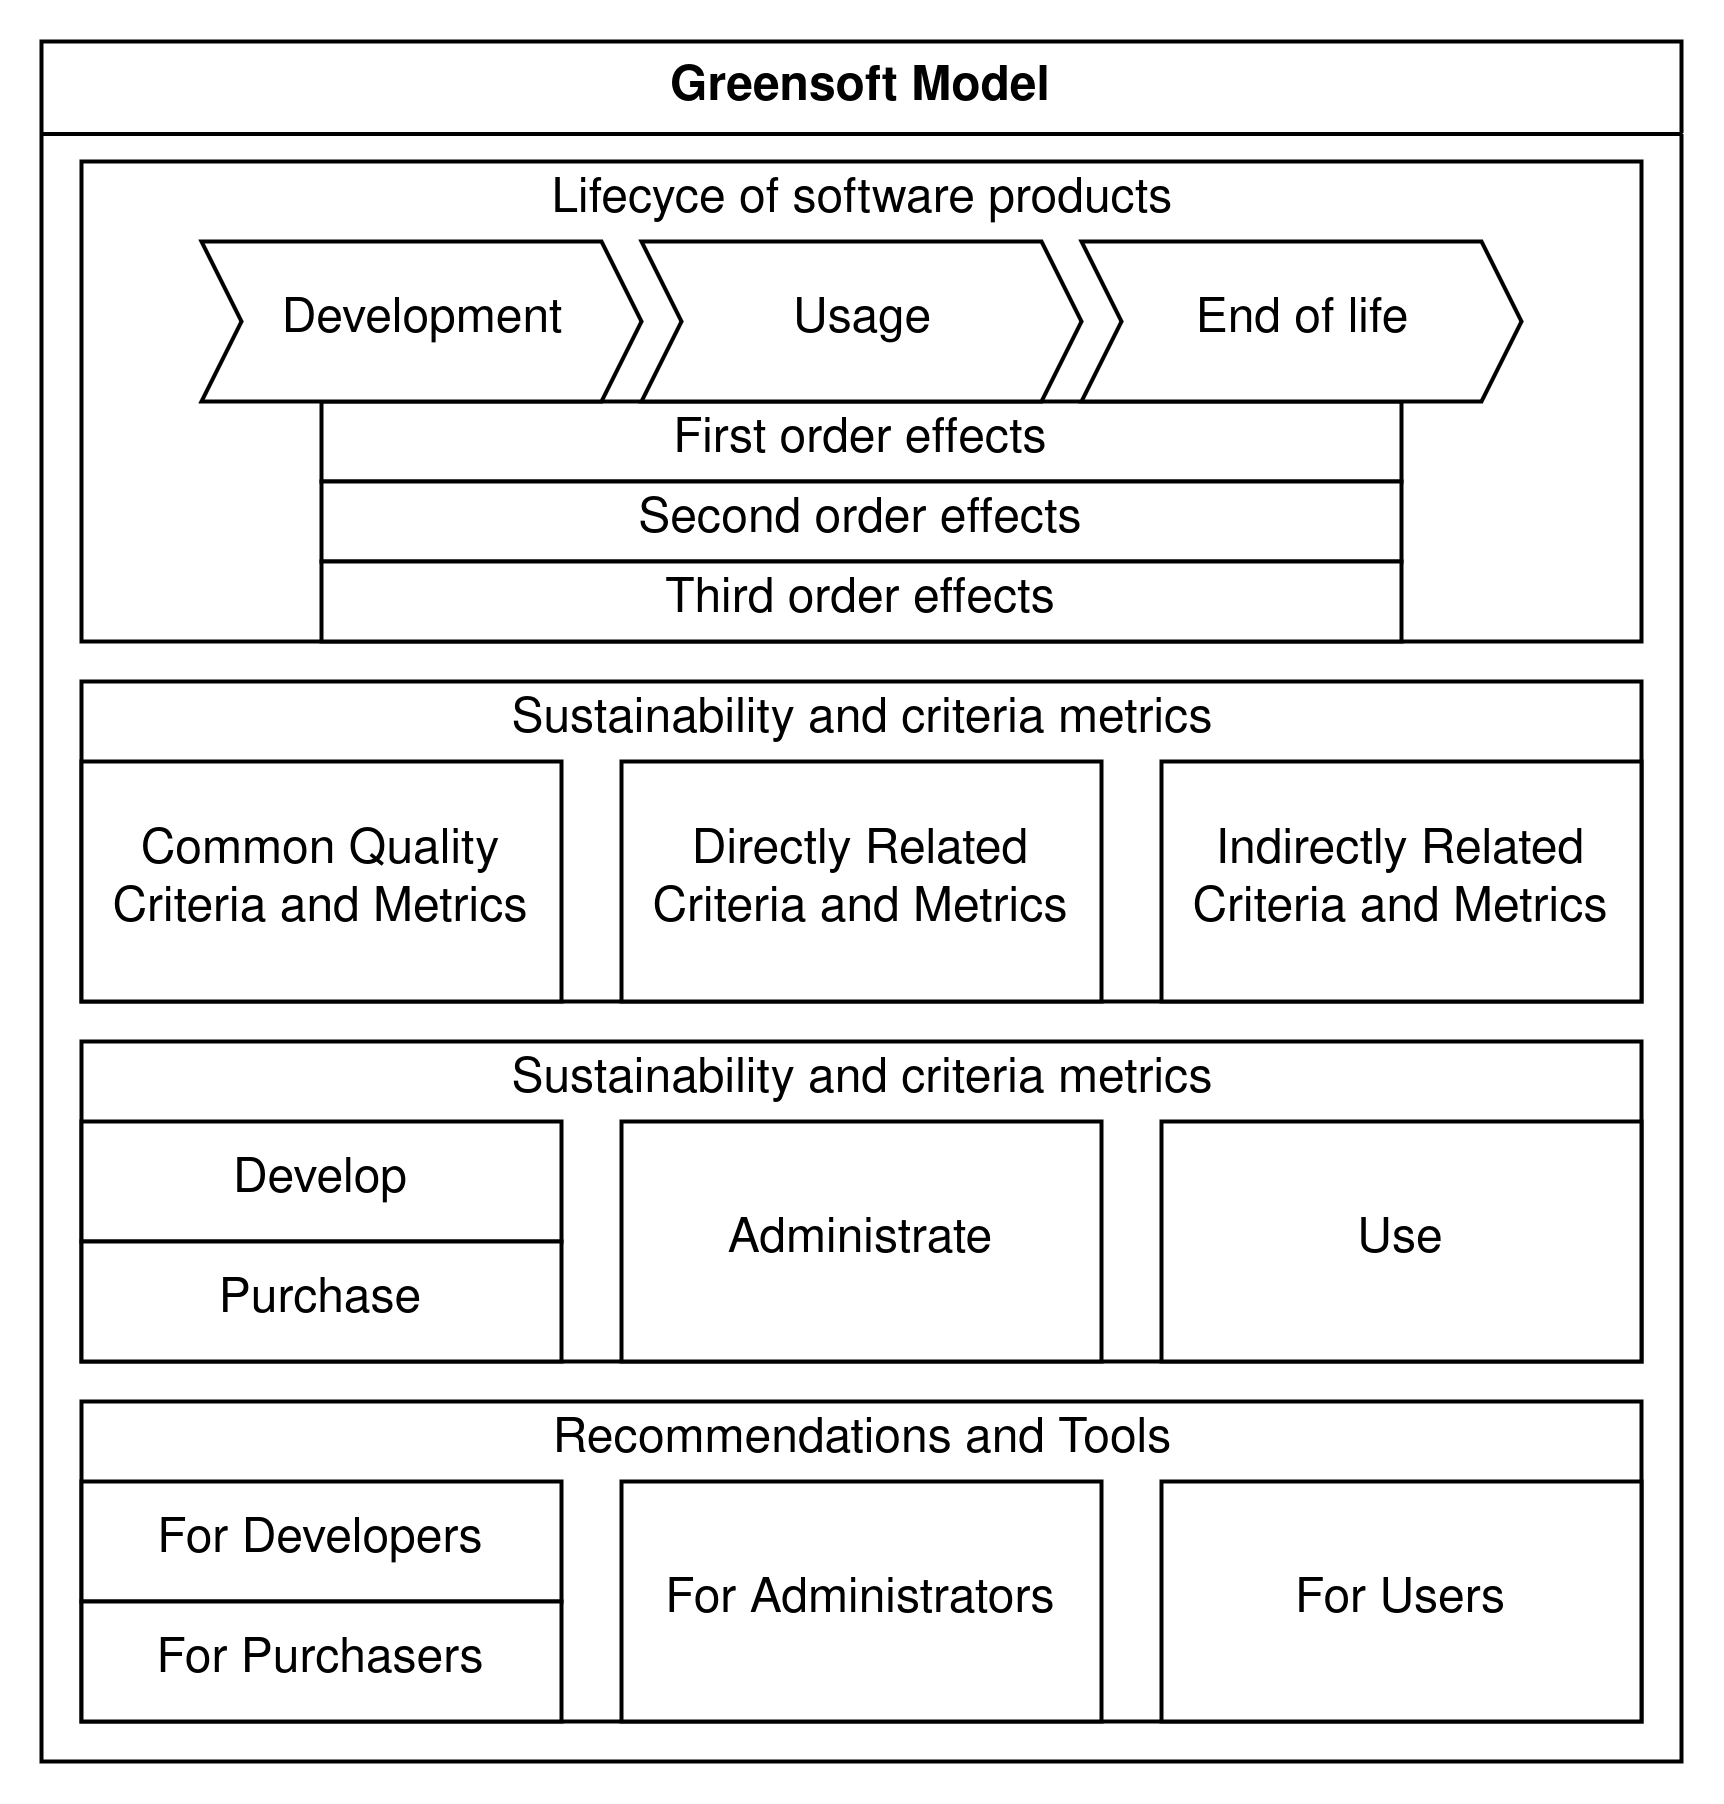
\includegraphics[width=\textwidth]{images/greensoft.png}
\centering
\end{figure}

\subsubsection{Life cycle of a software product}
The life cycle of software products is split into 3 different parts: development, usage, and end of life. All parts have first-, second-, and third-order effects on the sustainability of the software. First-order effects include direct effects of ICT supply. These include things such as performance and hardware requirements. Second-order effects include the effects of ICT usage. Third-order effects are the systemic effects of ICT. First-order effects are therefore in the \gls{greeninit}-category and second and third-order effects in \gls{greenbyit}- category~\cite{greensoft}. As this thesis is focused on the \gls{greeninit} category, first-order effects will be focused on here. The Life cycle of a software product is shown in Figure~\ref{lifecycle}.

\begin{figure}[H]
\caption{Life cycle of the software product}
\label{lifecycle}
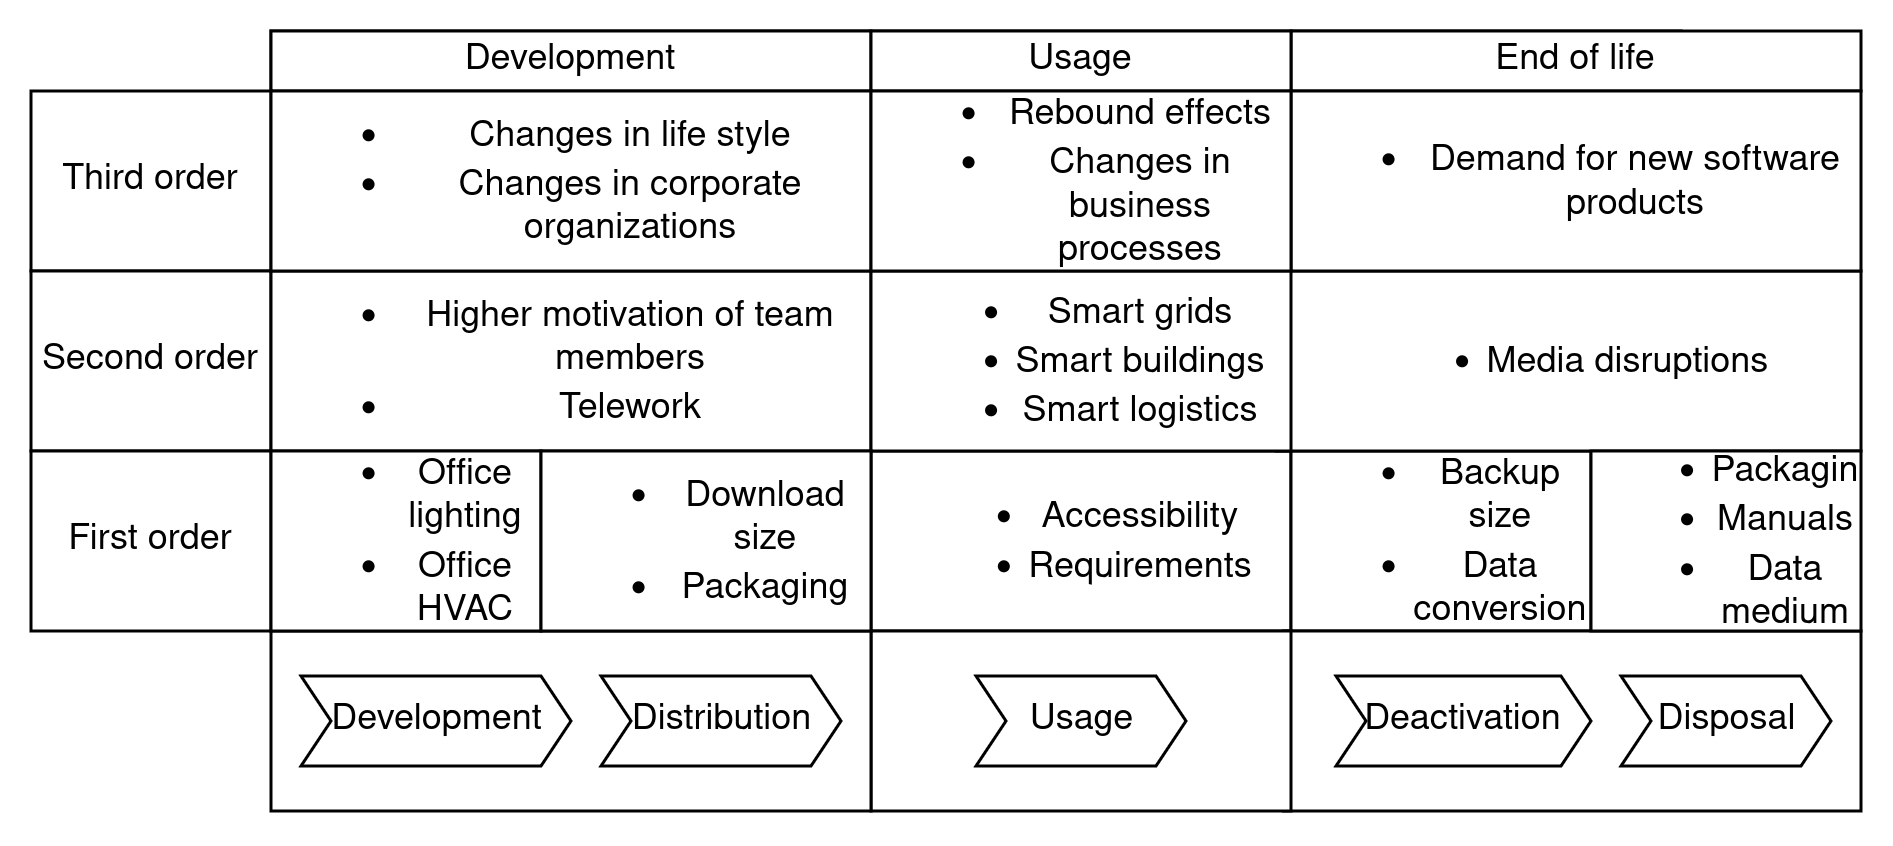
\includegraphics[width=\textwidth]{images/lifecycle.png}
\centering
\end{figure}

The development phase of the Greensoft model takes into account both development and distribution factors. These include office costs and conditions, commuting to work, business trips, and ICT energy usage. The distribution part includes things such as the size of the software, data formats, packaging, and transportation.

The usage part of the software is concerned with hardware requirements and overall energy consumption of the software and other resources required by it. The usage phase is the most affected by the software itself being as energy efficient as possible.

The final phase, end of life, is split into deactivation and disposal. Deactivation is concerned with preserving the data from the software and as such is affected by the backup size, format, and conversion of the data and long-term data storage. The disposal part on the other hand takes into account the data medium and packaging. This phase is used when at some point maintaining existing software can become too costly and a new software solution might be required. This can also be caused by changing business requirements or priorities. Energy consumption in this phase is mostly caused by saving and archiving data from the old software product because of legal restrictions or migrating data to the new software product. For these cases choosing the correct data format and compression method can make the migration easier and save time and disk space, which in turn reduces the energy needed.

\subsubsection{Indirect effects during development}
Some things affect the total energy use of the development that are not directly related to the software being made. These are called second and third-order effects~\cite{greensoft}. The office space used for working and how efficient it is regarding things such as heating and air conditioning are also factors. Some new building may even produce their energy with solar panels and be able to store it in batteries for later use. Indirect effects are mostly outside the scope of this thesis.

Remote working can also affect total energy consumption. Depending on the distance from home to the office and what is used to commute to work, it might be better to work remotely when possible and utilize different communication services to work in teams.

Development time and effects related to that should also be considered. The choice of the most efficient technologies might not be a net positive if developers are not familiar with them and developing the software takes longer than with familiar technologies.

Organizations can affect how people commute by providing public transportation tickets for workers or otherwise encouraging using public transport or non-polluting vehicles such as bicycles. The viability of these options is somewhat dependent on the distance between the workplace and the home of the employee.

\subsubsection{Sustainability Criteria and Metrics}
The model presents different quality properties that can be observed in different phases of the software lifecycle. The development phase lists modifiability, reusability, predictability, and efficiency as properties. Usage phase on the other hand lists portability, stability, performance, dependability, usability, and accessibility.

The model states that hardware lifetime should be maximized in order to prevent costs from replacing it. For this purpose the performance and portability of the software are important as performance helps maximize the lifetime of hardware and portability makes it easier to switch hardware when replacing it becomes necessary.

Energy efficiency is also an important metric. Energy efficiency is affected by more than just the runtime performance of the software. For example, lowering performance requirements or required service quality can help in reducing the overall energy usage of the software.~\cite{greensoft}

\subsubsection{Procedure models}
The procedure models presented in the model are split into develop, purchase, administrate, and use submodels.

The development model proposes adding sustainability review and preview, process assessment, sustainability journal, and sustainability retrospective to the software development process. The idea behind this is that these can be added to any software development process that is iterative.

The purchase model mostly focuses on procurement processes. Purchasing and procurement processes can define criteria that require measurement of energy efficiency, specific features such as those presented in the Criteria for software systems~\cite{kriteeripankkiSoftwareServices}.

The administrator model focuses on allowing administrators to install, configure, and monitor the software. This includes allowing administrators to check the energy and resource consumption of the software.

The use model focuses on how the users use the software. This is affected by the design of the software as well as the features in it that allow users to customize their experience. Displaying data on software resource usage and energy consumption may also affect the usage of the software by users.

\subsubsection{Recommendations and tools}
The model recommends making tools and recommendations available for different user groups to monitor and improve their energy usage. These tools and recommendations can include checklists, best practices, and guides for different user groups on how to use software more efficiently. This could be an optimization guide for developers, for administrators a tool that allows them to make infrastructure choices based on sustainability, and for users, a tool that allows them to configure their system's behavior regarding performance and energy consumption.~\cite{greensoft}

\subsection{A Green Model for Sustainable Software Engineering}\label{greenmodelforsustainable}
Mahmoud and Ahmad present a two-level model for creating green software and measuring the greenness of the software~\cite{greenmodelforsustainable}. The first level of the model aims to present an agile and green software development process. The second level presents different ways to measure the greenness of the software using existing tools and methods.

\subsubsection{Level 1}
The first level is divided into seven stages that represent different parts of the software engineering process. These stages are shown in Figure~\ref{level1}. 

\begin{figure}[H]
\caption{Level 1 of the green model for sustainable software engineering~\cite{greenmodelforsustainable}}
\label{level1}
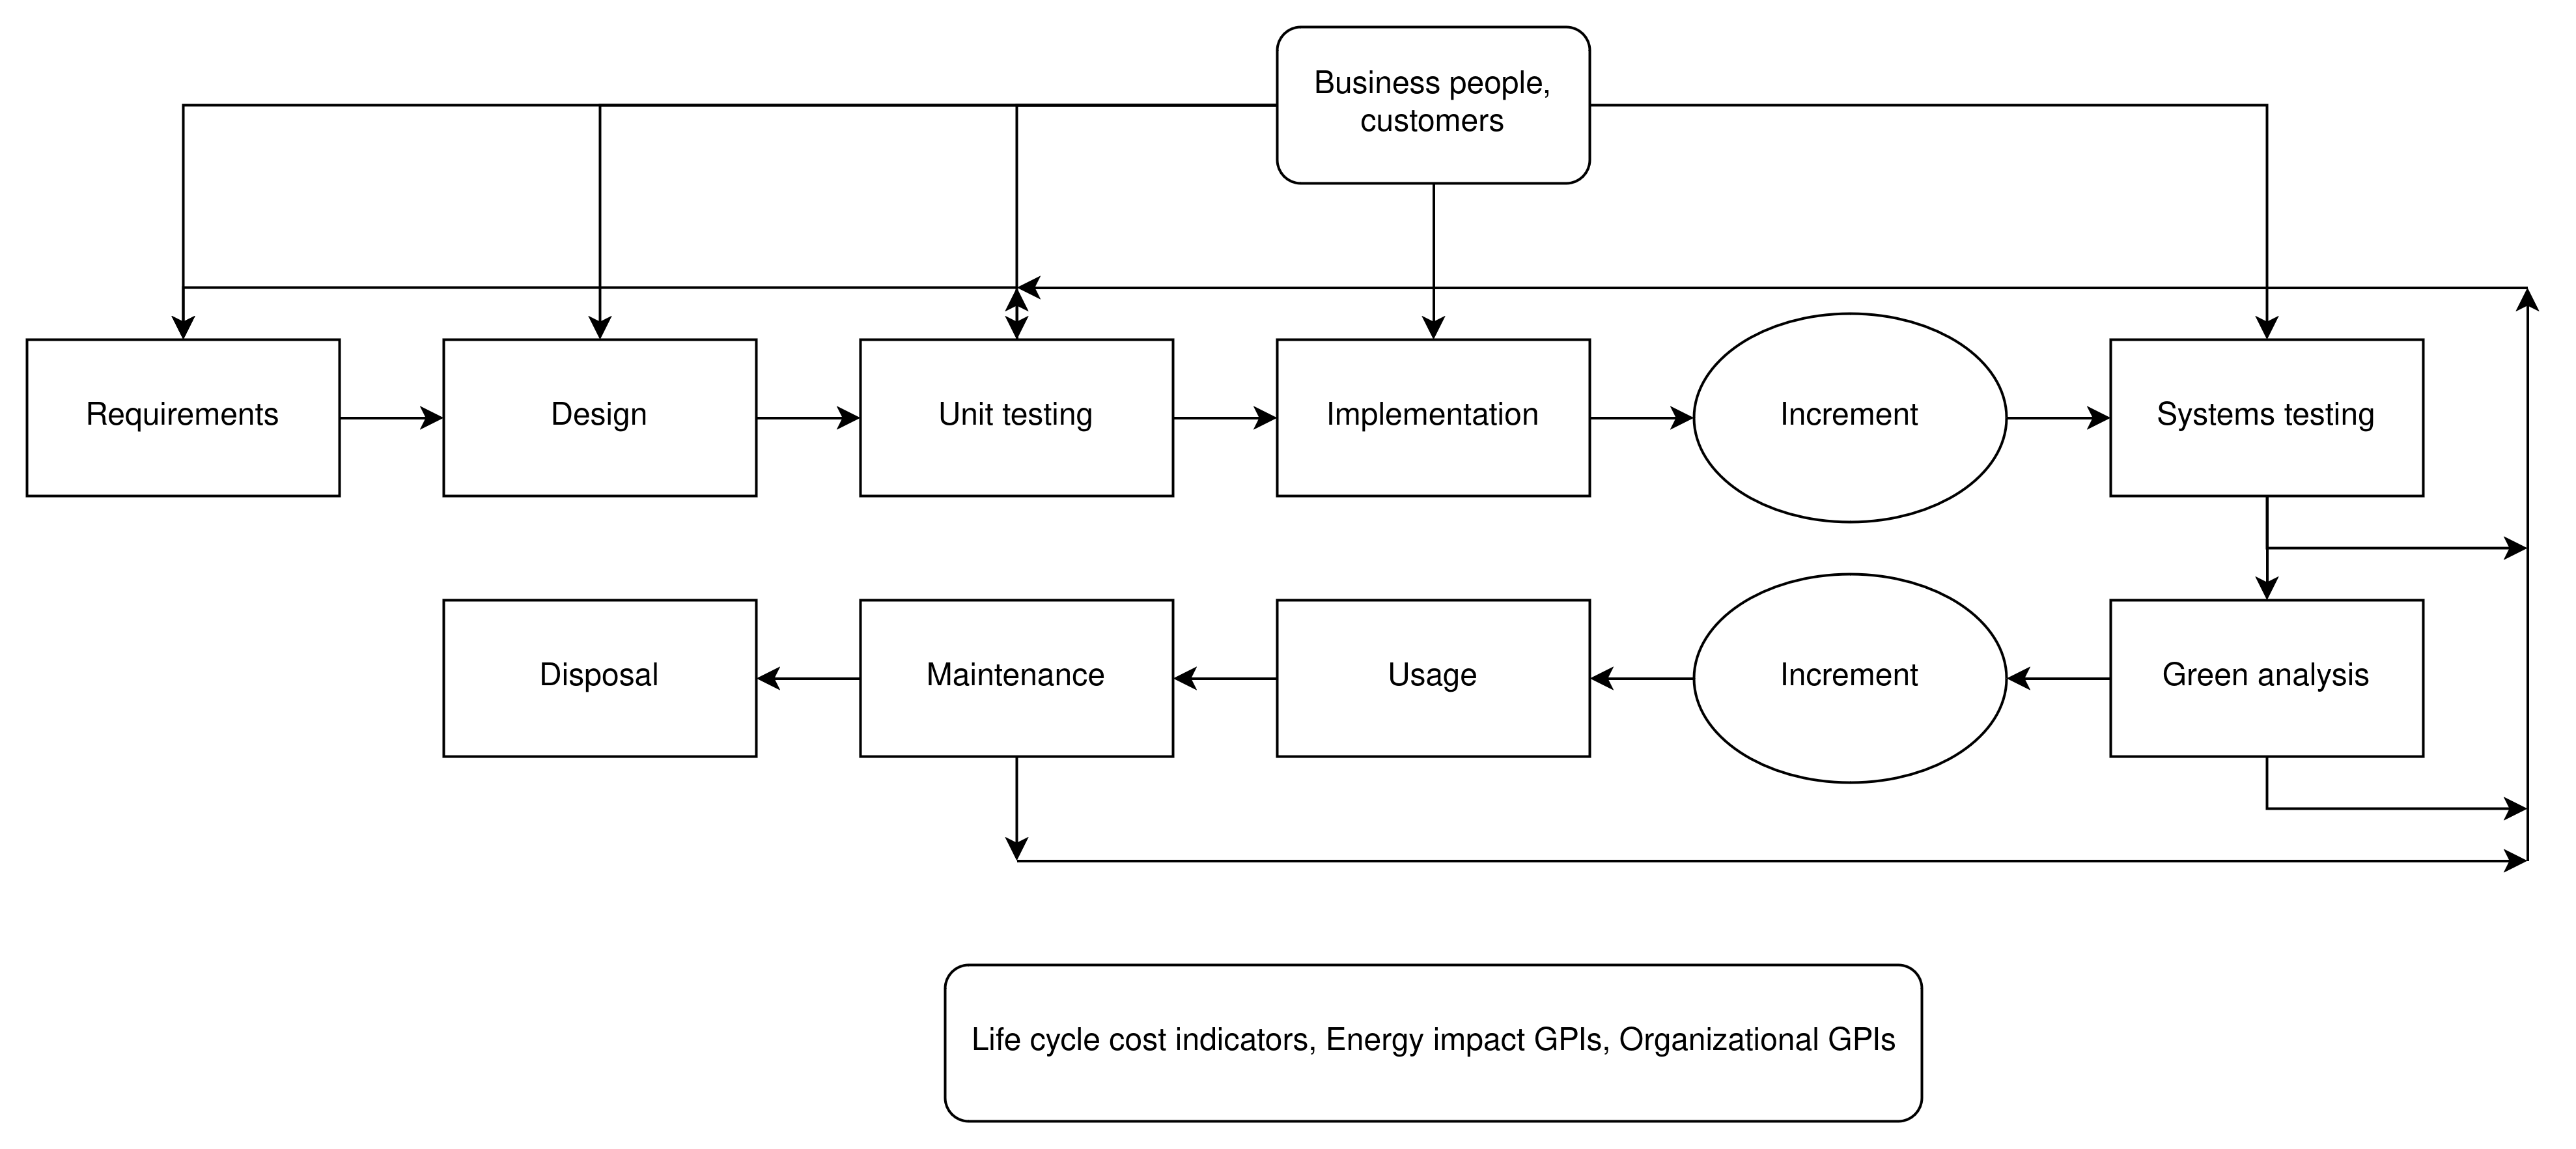
\includegraphics[width=\textwidth]{level1.png}
\centering
\end{figure}

The first stage is requirements engineering. This stage aims to determine the feasibility of the system if the system can solve the specific problem, create an outline for services to be provided, order the services, analyze the risk in terms of energy, and finally test the requirements. This stage is inspired by extreme programming conventions of requirements testing.

The design and implementation stages are used to create system architecture based on requirements. This stage includes guidelines for designing environmentally sustainable software. The guidelines mention using efficient algorithms based on the used data structures, programming languages, and hardware. The guidelines also mention that systems should stick to design and be as small as possible to avoid unnecessary lines of code. Frameworks and libraries are mentioned as potentially detrimental as they add more layers to software and might make it more inefficient.

The third stage is the testing stage which aims to discover defects in software functionality or meeting requirements. Tests should be developed early in the project. The paper presents metrics including fault tolerance, failure management, and testability for measuring the environmental impact of testing on software.

The fourth stage is analysis which aims to measure the energy usage of the software itself using metrics such as CPU usage, performance tests such as benchmarks and debug logs. Hardware may also support specific power measuring functions that could be used.

The fifth stage is usage which takes into account how users use the program. Software should aim to be simple and allow users to perform the minimum amount of actions for software to fulfill its purpose. Software should also support power management features such as using minimal power when idle.

The sixth stage is maintenance. This step is concerned with the maintainability of the software such as required access and knowledge to perform it and the amount and quality of documentation available for the software.

The final stage is disposal and it is concerned with how well the software can be recycled and reused in other software, how hardware can be recycled or repurposed, and how efficiently is migrating to the next software product.~\cite{greenmodelforsustainable}

\subsubsection{Level 2}
The second level introduces different tools for creating, measuring, and using energy-efficient software. This includes operating systems, application frameworks, energy usage measurement software, virtualization technologies for maximizing hardware use, and \gls{greenbyit} products that are used to help reduce energy consumption. The second level is shown in Figure~\ref{level2}.~\cite{greenmodelforsustainable}

\begin{figure}[H]
\caption{Level 2 of the green model for sustainable software engineering~\cite{greenmodelforsustainable}}
\label{level2}
\includegraphics[width=\textwidth]{level2.png}
\centering
\end{figure}

\subsubsection{Tools and Metrics}
The paper presents metrics for measuring the impact of the software being developed. These metrics are presented in Figure~\ref{metrics}. The GPI metrics are divided into IT resource usage, applications life cycle KPIs, Energy impact, and Organizational GPIs.

IT resource usage metrics take into account the resource usage of the software, Application lifecycle takes into account the development and configuring costs. The energy impact on the other hand takes into account the impact of data centers. The organizational GPIs include organizational factors. ~\cite{greenmodelforsustainable}

\begin{figure}[H]
\caption{Metrics for green software of the green model for sustainable software engineering~\cite{greenmodelforsustainable}}
\label{metrics}
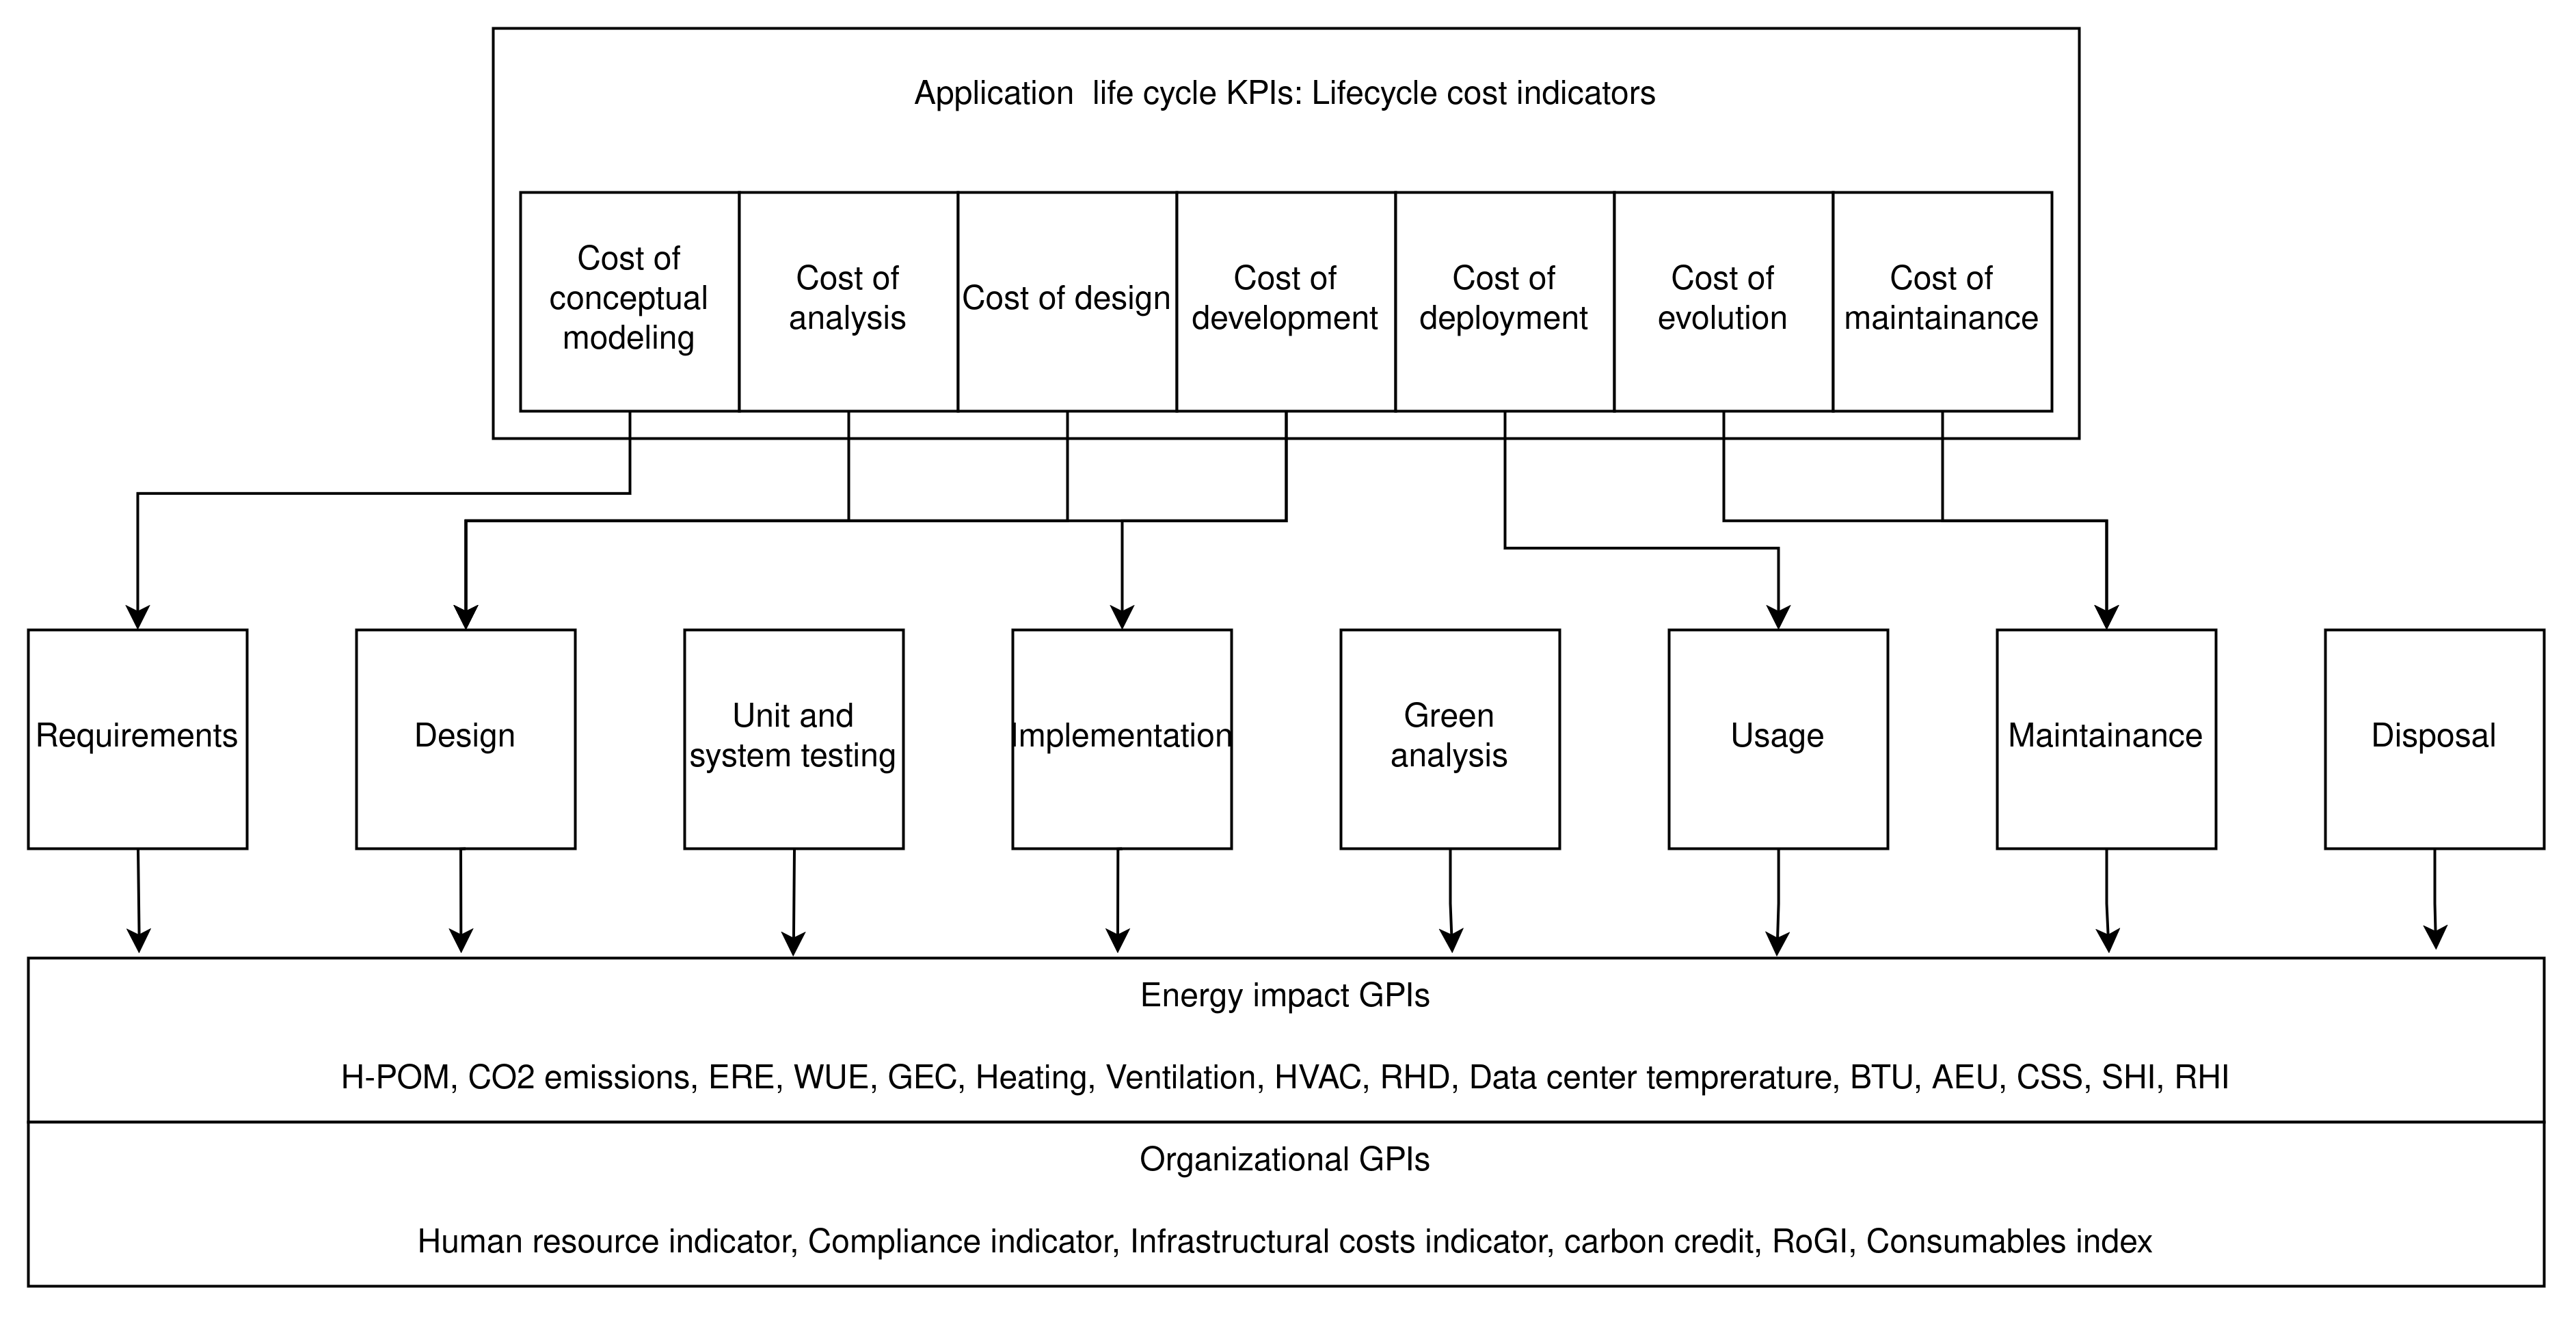
\includegraphics[width=\textwidth]{images/greenmetrics.png}
\centering
\end{figure}

\subsection{Green Lean process}\label{waste}
Ibrahim, Sallehudin, and Yahaya explore using lean methods to reduce waste in software development processes. It presents preliminary work for Green Lean Development components. The study considers Software waste, meaning incomplete work, unnecessary features, lost knowledge, hand-offs, task switching, delays, and defects, and theorizes that reducing them using lean methods will lead to greener software. Therefore sustainable software processes should strive to eliminate this waste. The paper shows that developing the Green Lean Model combines energy efficiency, waste reduction, and sustainable design~\cite{waste}. The process is shown in Figure~\ref{lean}.

\begin{figure}[H]
\caption{Green lean process~\cite{waste}}
\label{lean}
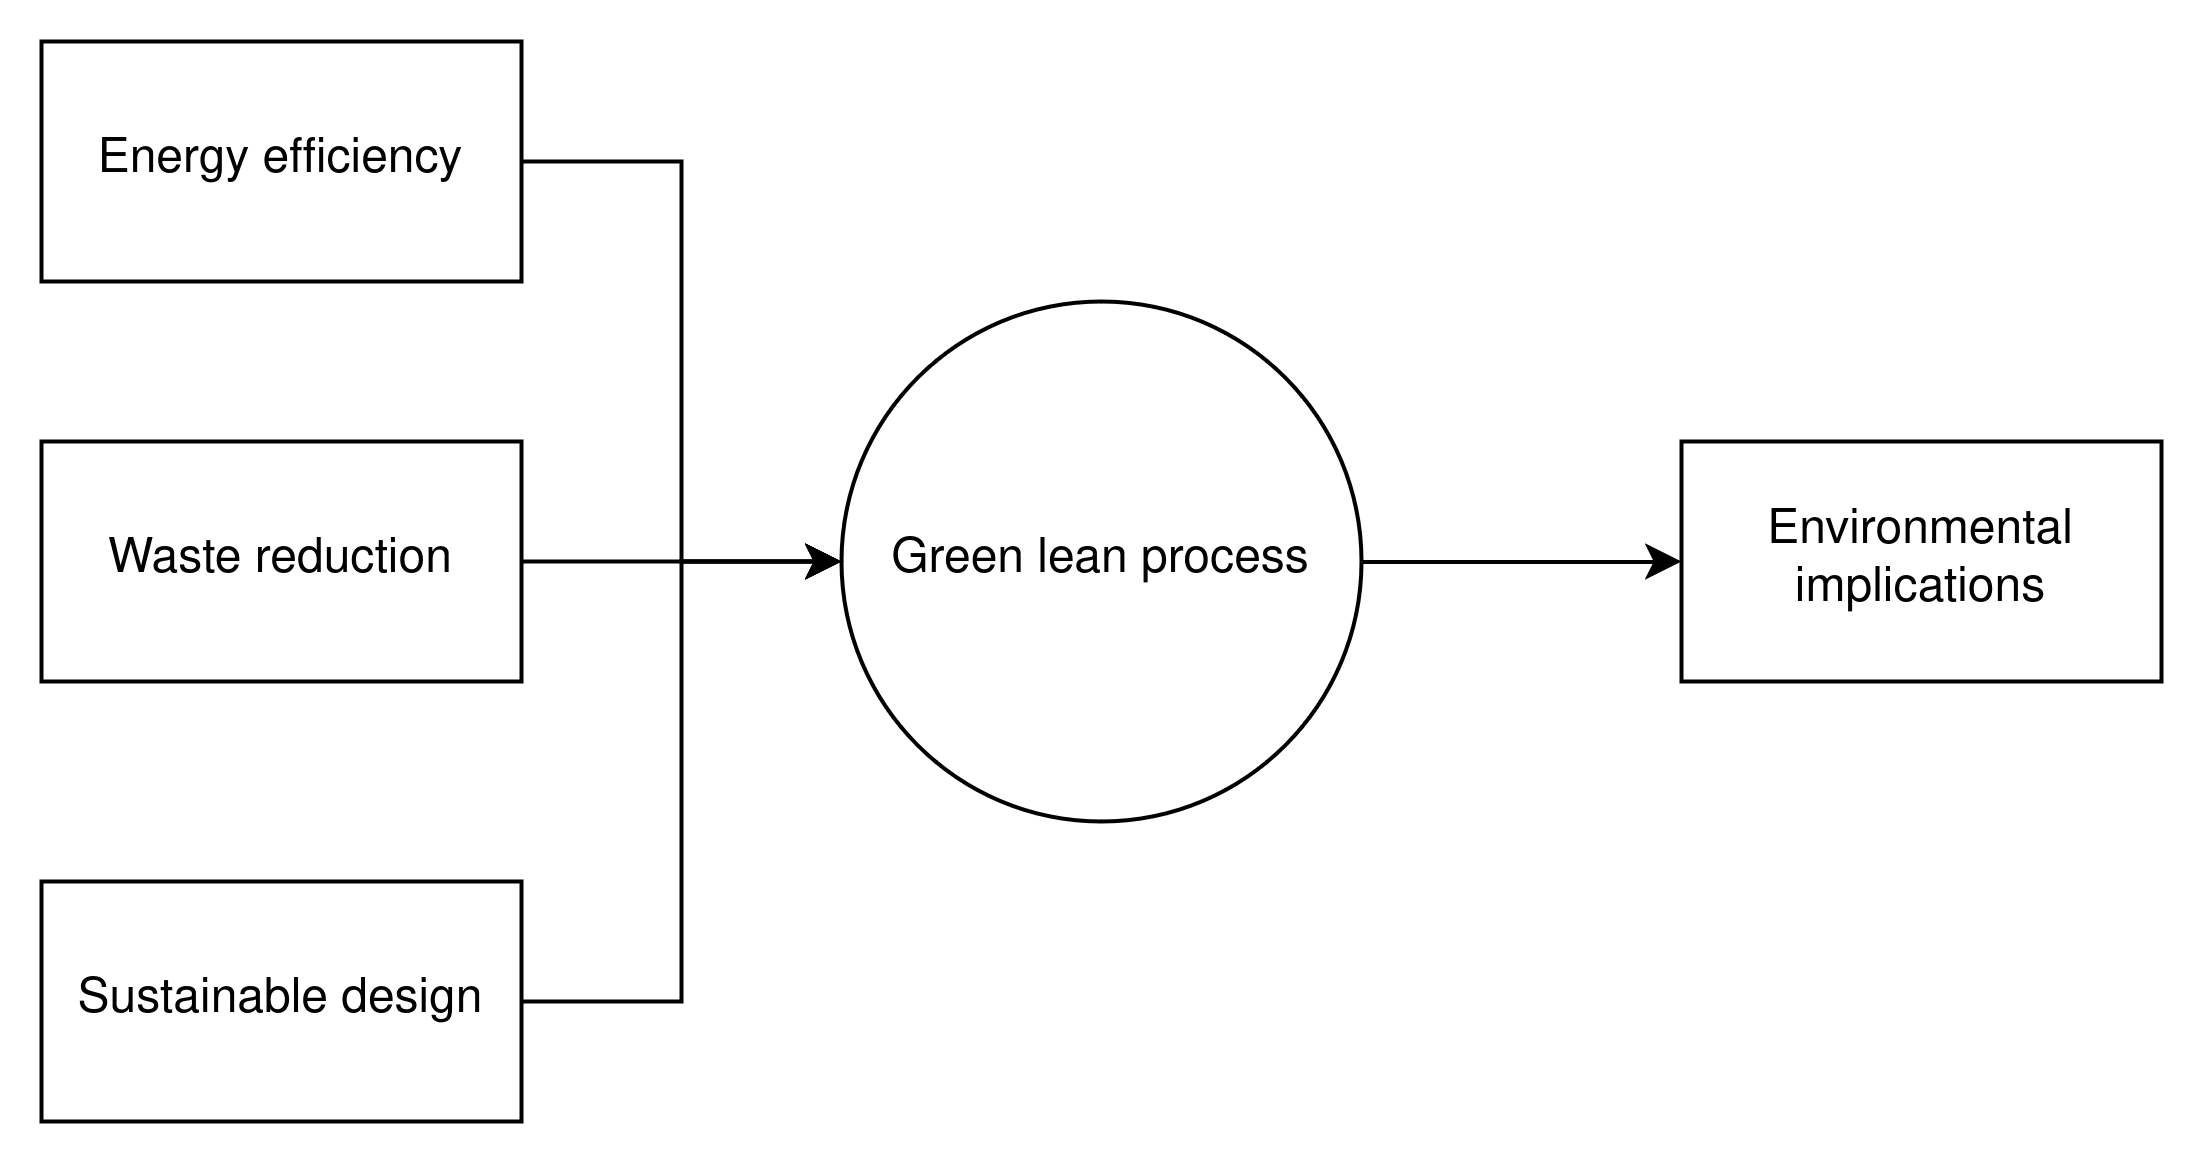
\includegraphics[width=\textwidth]{lean.png}
\centering
\end{figure}
